        \clearpage
        \begin{figure*}[ht]
            \pdfbookmark[2]{ID 02}{figure_id_02}
        	\centering
            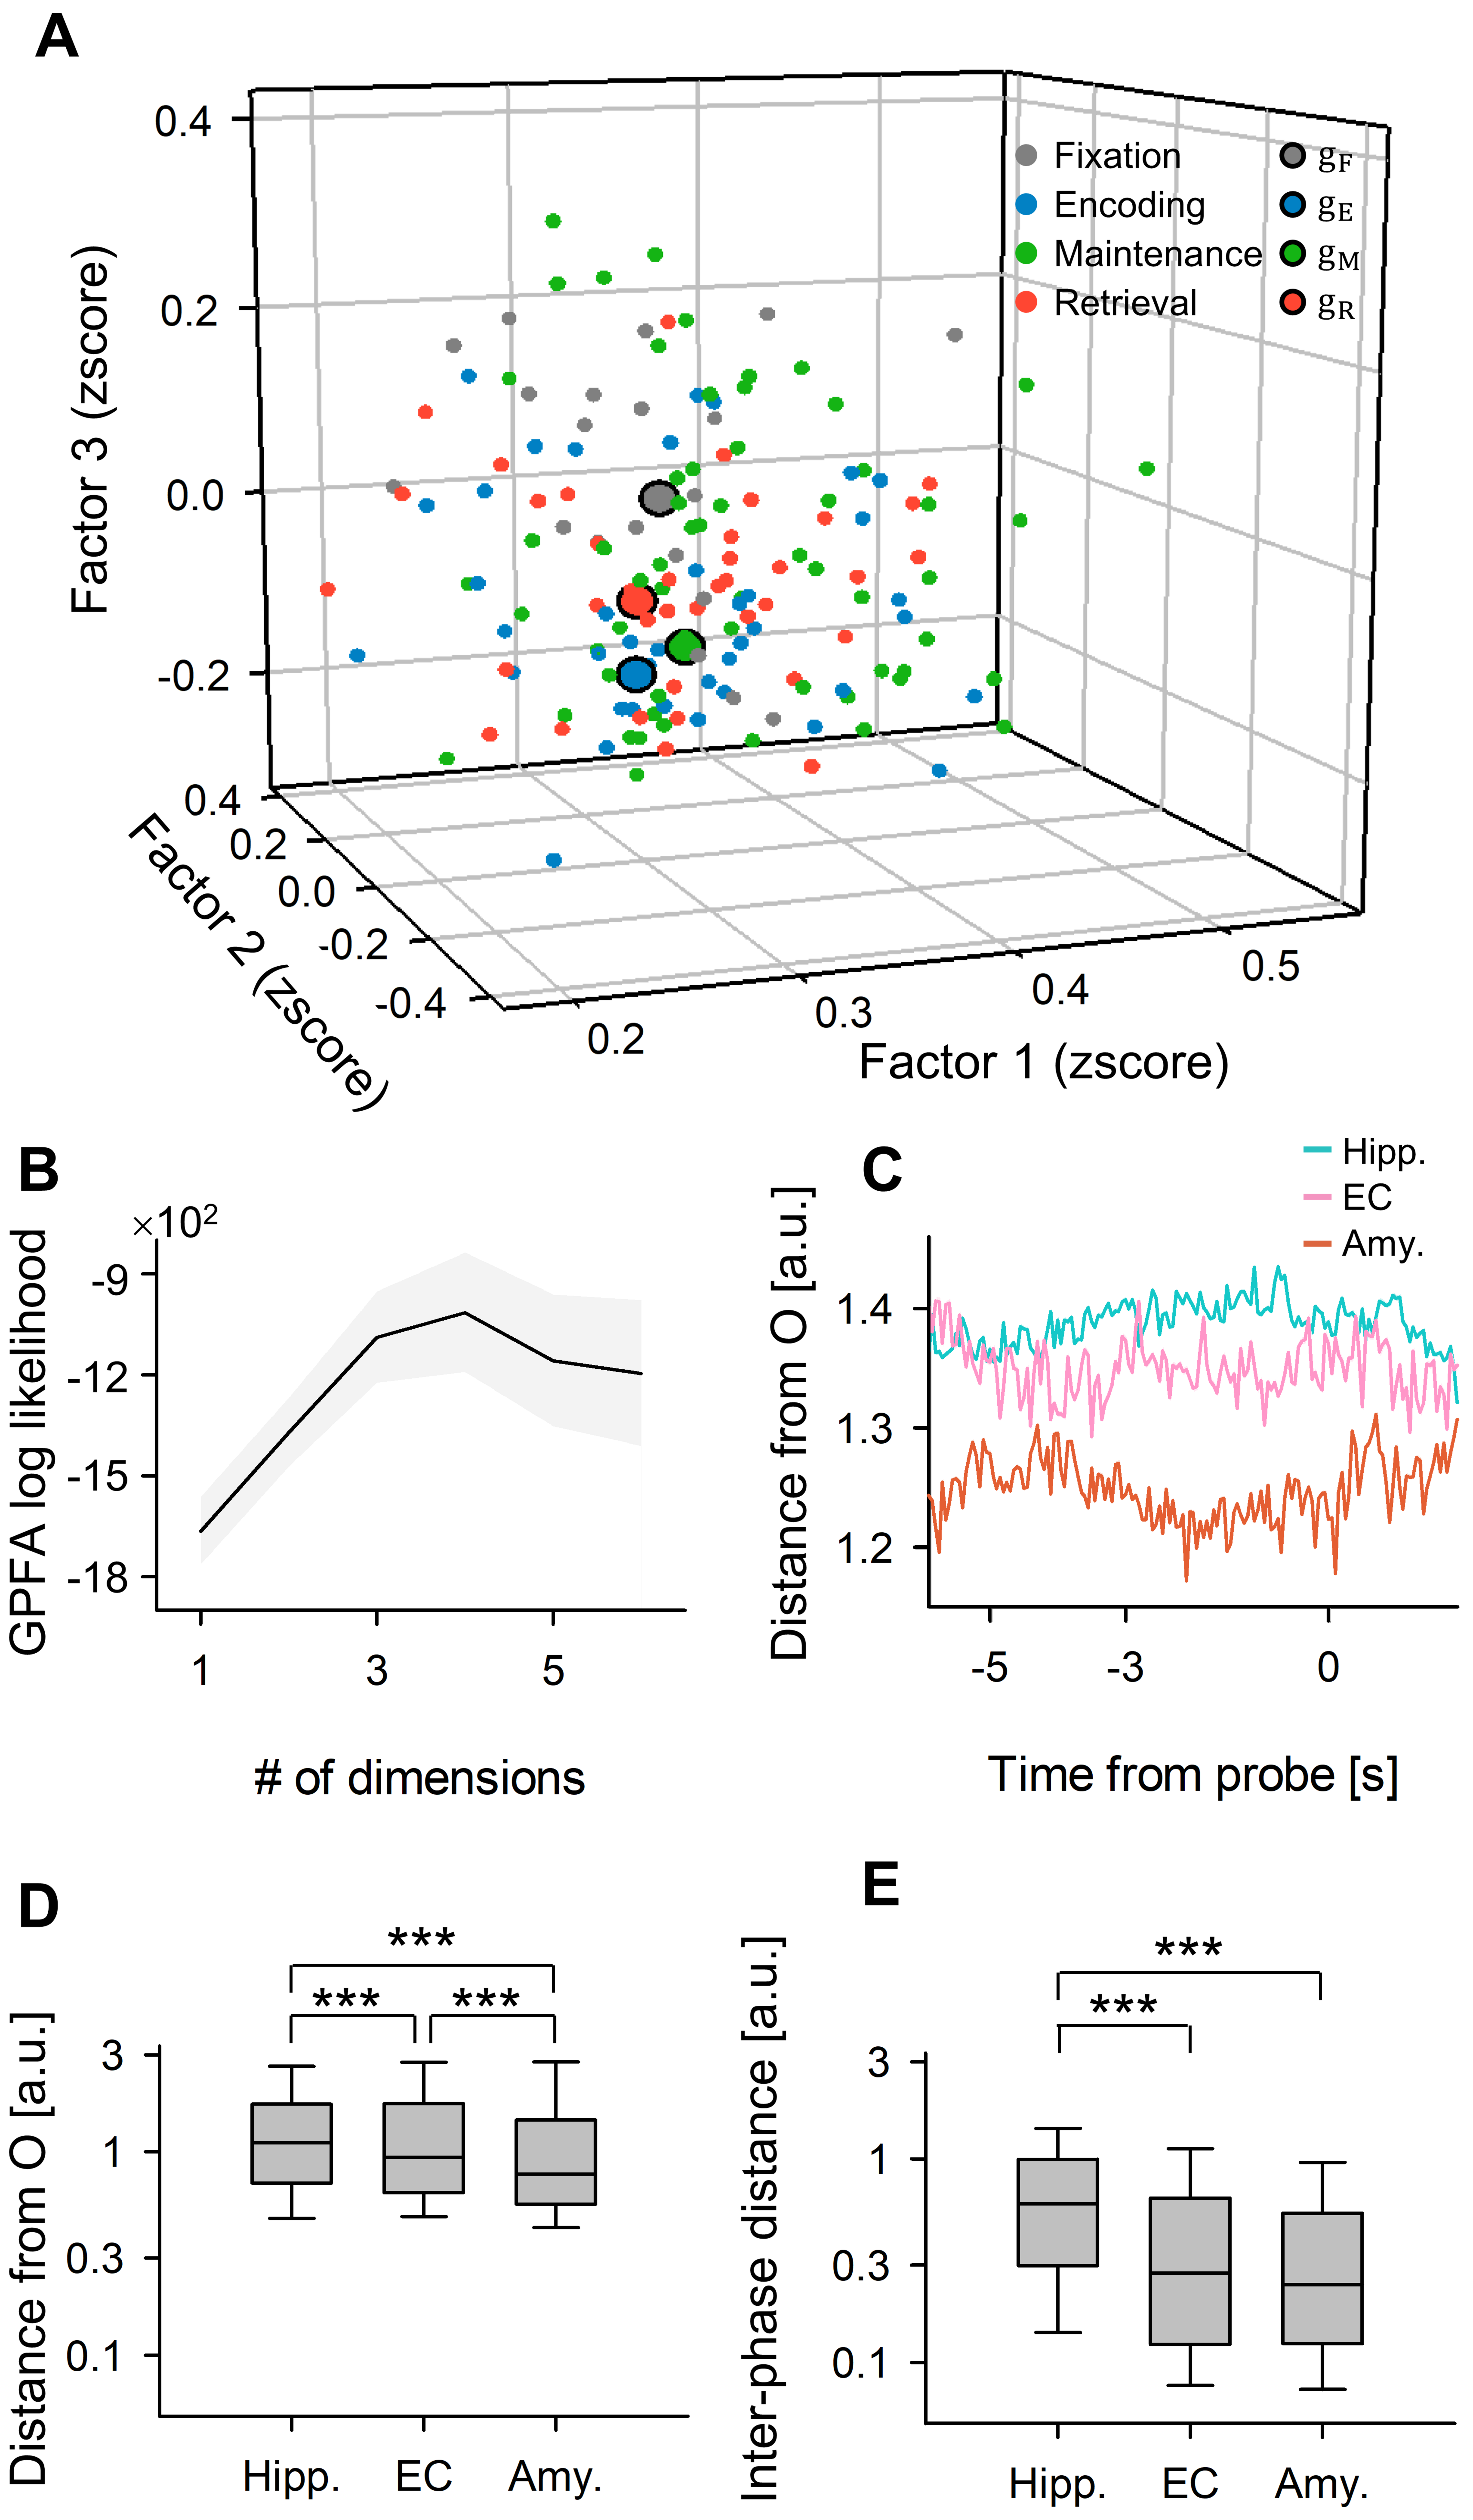
\includegraphics[width=0.5\textwidth]{./src/figures/png/Figure_ID_02.png}
        	\caption{\textbf{
State-Dependent Neural Trajectory of Hippocampal Neurons
}
\smallskip
\\
\textbf{\textit{A.}} Neural trajectories (NTs) depicted as a point cloud within the first three-dimensional factors derived from GPFA \cite{yu_gaussian-process_2009}. The smaller dots represent 50-ms NT bins, and the larger dots with \textit{black} edges denote the geometric medians for each phase in the Sternberg working memory task: fixation ($\mathrm{\lVert g_{F} \rVert}$, \textit{gray}), encoding ($\mathrm{\lVert g_{E} \rVert}$, \textit{blue}), maintenance ($\mathrm{\lVert g_{M} \rVert}$, \textit{green}), and retrieval ($\mathrm{\lVert g_{R} \rVert}$, \textit{red}). \textbf{\textit{B.}} The figure presents the log-likelihood of the GPFA models versus the number of dimensions used to embed multi-unit spikes found in the medial temporal lobe (MTL) regions. Specifically, the elbow method identified three as the optimal dimension. \textbf{\textit{C.}} This panel displays the distance of the NTs from the origin ($O$) for the hippocampus (Hipp.), entorhinal cortex (EC), and amygdala (Amy.), plotted against the time elapsed from the probe onset. \textbf{\textit{D.}} The NT distance from $O$ within the MTL regions is shown. The hippocampus has the greatest distance, followed by the EC and the Amygdala. \textbf{\textit{E.}} The box plot illustrates inter-phase NT distances within the MTL regions.
}
% width=0.5\textwidth
        	\label{fig:02}
        \end{figure*}
